%---------------------------------------------
%	PACKAGES AND OTHER DOCUMENT CONFIGURATIONS
%---------------------------------------------
\documentclass[
	letterpaper, % Letter Paper (Required for 4490Z)
	10pt, % Font Size
	%twoside, % Commented out for fixed headers/footers
]{journalArticle}

% BibLaTeX bibliography file
\addbibresource{references.bib}

% Running Header
\runninghead{Gavigan, Riley}

% Footer Content
\footertext{}

% Page Counter Starting Number
\setcounter{page}{1}

%---------------------------------------------
%	TITLE SECTION
%---------------------------------------------
\title{Explaining embedding vector results for alignments\\ Thesis proposal (CS 4490Z)}

% Authors are listed in a comma-separated list with superscript numbers indicating affiliations
% \thanks{} is used for any text that should be placed in a footnote on the first page, such as the corresponding author's email, journal acceptance dates, a copyright/license notice, keywords, etc
\author{
	Riley Gavigan\textsuperscript{1}, Lucian Ilie\textsuperscript{1}\thanks{Thesis supervisor. Bioinformatics Lab - csd.uwo.ca/\textasciitilde ilie/lab.html}, Nazim Madhavji\textsuperscript{1}\thanks{Course supervisor}\\
}

% Affiliations are output in the \date{} command
\date{{\footnotesize{\textsuperscript{\textbf{1}}Department of Computer Science, University of Western Ontario, London, N6A 5B7, Ontario, Canada\\}}\vspace{1em}November 27, 2023\\}

% Full-width General Abstract
\renewcommand{\maketitlehookd}{%
	\begin{abstract}
		\noindent The proposed E-score alignment scoring method \autocite{Ashrafzadeh:2023} generates results that further research will explore, leading to insight for performance improvement. Cosine similarity results generated by the models were mostly positive instead of being randomly distributed. Exploration of this distribution will lead to a better understanding of the different models and the embedding vectors being produced. Different embedding models also differ greatly in performance with varying mean ranges. From this research, insight will be obtained to improve embedding performance and transformer model architecture.
	\end{abstract}
}
%------------------------------------------
\begin{document}
\maketitle % Output the title section
%---------------------------------------------
%	STRUCTURED ABSTRACT
%---------------------------------------------
\section{Structured Abstract}

% Context and Motivation
\subsection{Context and motivation}
The \textit{E}-score protein alignment scoring method \autocite{Ashrafzadeh:2023} outperforms state-of-the-art methods, supported by comparing ProtT5 \autocite{Elnaggar:2021} \textit{E}-score results with BLOSUM62 \autocite{Henikoff:1992}.

This research aims to understand \textit{E}-score results, building upon the observation that mean cosine similarity results between two embeddings are not evenly distributed.

By understanding the underlying causes of the observed results, we can improve the \textit{E}-score method. Insights can be used to fine-tune the transformer models \autocite{Elnaggar:2021, Rives:2021} and performance of embeddings.

% Research Questions
\subsection{Research questions}
\begin{itemize}
    \item{What properties of embeddings produce better cosine similarity results?}
    \item{Why does ProtT5 produce the best embeddings?}
    \item{Why do cosine similarity results primarily fall within a positive range?}
    \item{How can the underlying models be fine-tuned to produce better embeddings?}
\end{itemize}

% Principal Ideas
\subsection{Principal ideas}
Positive cosine similarity results imply the produced embeddings are mostly similar. Comparing different embedding types will provide insight into their distributions. Through these comparisons, conclusions about properties that improve \textit{E}-score results can be drawn.

% Research Methodology
\subsection{Research methodology}
This research is a data science investigation to obtain insight about the embeddings and cosine similarity results in the \textit{E}-score method.

\noindent Research resources:
\begin{itemize}[noitemsep]
    \item{\href{https://github.com/rgavigan/e-score}{\textit{E}-score analysis notebook}}
    \item{\href{https://github.com/agemagician/ProtTrans/tree/master/Fine-Tuning}{ProtT5 fine-tuning notebook}}
    \item{\href{https://aws.amazon.com/sagemaker/studio/}{SageMaker Studio} and \href{https://www.csd.uwo.ca/~ilie/lab.html}{Bioinformatics Lab} compute power}
\end{itemize}

% Anticipated Type of Results
\subsection{Anticipated type of results}
This study primarily aims to obtain insight and knowledge for the \textit{E}-score method, specifically:
\begin{itemize}
    \item{Knowledge about the distributions of different embedding types}
    \item{Knowledge about the cosine similarity between embeddings}
    \item{Insight to fine-tune and improve the available models}
    \item{Findings that can be reproduced for Natural Language Processing models and embeddings}
\end{itemize}

% Anticipated Novelty
\subsection{Anticipated novelty}
By building upon a novel method for scoring protein alignments using cosine similarity \autocite{Ashrafzadeh:2023}, anticipated results from this research will be novel conclusions that can further be explored and built upon.

% Anticipated Impact of Results
\subsection{Anticipated impact of results}
Improvements in transformer models for the \textit{E}-score alignment scoring method can be made through the insight this research finds. Any anticipated improvements would also be applicable to Natural Language Processing Models, such as T5 \autocite{Raffel:2020}.

%---------------------------------------------
%	BACKGROUND AND RELATED WORK
%---------------------------------------------
\section{Background and Related Work}

% Protein Transformers
\subsection{Protein transformers}
The \textit{E}-score alignment method depends on several protein transformer models (shown in Table \ref{tab:transformers}) to generate embeddings for a protein sequence prior to calculating cosine similarity. These transformers include ProtT5, ProtBert, ProtAlbert, and ProtXLNet\footnote{https://github.com/agemagician/ProtTrans} from the ProtTrans project \autocite{Elnaggar:2021}, as well as ESM1b and ESM2\footnote{https://github.com/facebookresearch/esm} from the Meta Fundamental AI Research Protein (FAIR) Team \autocite{Rives:2021}.

\begin{table} % Single column table
	\caption{Transformer models available in the \textit{E}-score method.}
	\centering
	\begin{tabular}{ |c|c|c| }
		\toprule
		Model & Embedding Dim & Pre-Trained On \\
		\midrule
		ProtT5 & 1024 & UniRef50 \\
		ProtBert & 1024 & UniRef100 \\
		ProtAlbert & 4096 & UniRef100 \\
            ProtXLNet & 1024 & UniRef100 \\
            ESM1b & 1280 & UniRef50 \\
            ESM2 & 1280 & UniRef50 \\
		\bottomrule
	\end{tabular}
	\label{tab:transformers}
\end{table}

The ProtT5 model's average \textit{E}-score performance was the most similar to the BLOSUM62 matrix, shown in Figure \ref{fig:escoreheatmap}. BLOSUM62 is the best-performing old method for scoring alignments \autocite{Ashrafzadeh:2023}, making it a valuable comparison for the \textit{E}-score models. ProtT5 serves as a strong benchmark to compare other models to in understanding embedding \textit{E}-score performance.

% Embedding Vectors
\subsection{Embedding vectors}
The embedding vector produced for a given protein sequence varies based on the model that was used. For example, the embedding for a protein sequence of 310 residues using ProtT5 will have the dimensions [310, 1024]. The embedding dimension outlined in Table \ref{tab:transformers} determines the columns of the embedding vector. The dimensionality of these vectors represents the number of features encoded in the embedding, and is a fixed value for a given model.

% E-Score Calculations
\subsection{\textit{E}-score calculations}
The embeddings produced for a model, calculated in Equation \ref{eq:embedding}, are used as the input to calculate the cosine similarity.

\begin{equation}
    E(P) = GetEmbeddings(Model = ProtT5)
    \label{eq:embedding}
\end{equation}

Calculating the cosine similarity between two vectors \(B = (B_i)_{i=1..n}\) is shown in Equation \ref{eq:cossim}.

\begin{equation}
	CosSim(A, B) = cos(\theta) \equiv \frac{A \cdot B}{\Vert A \Vert \Vert B \Vert} \equiv \frac{\sum\limits_{i=1}^{n} A_iB_i}{\sqrt{\sum\limits_{i=1}^{n} A_i^2}\sqrt{\sum\limits_{i=1}^{n} B_i^2}}
	\label{eq:cossim}
\end{equation}

\textit{E}-score is calculated by taking the cosine similarity between the embedding vector for two residues (\(i, j\)), shown in Equation \ref{eq:escore} where \(P_1\) and \(P_2\) are proteins \autocite{Ashrafzadeh:2023}.

\begin{equation}
    \textit{E}\mbox{-}score(i,j) = CosSim(E(P_1)_i, E(P_2)_j)
    \label{eq:escore}
\end{equation}

%---------------------------------------------
%	RESEARCH GOAL AND OBJECTIVES
%---------------------------------------------
\section{Research Goal and Objectives}
\textbf{Goal: }Obtain significant insight about the \textit{E}-score results and the differences between different models, leading to improvement of both the embedding performance and the embeddings being generated by the models.

Insight about performance differences between models has a significant impact outside of the \textit{E}-score method. These models are used extensively for other purposes and insight that can lead to performance improvements is important to the research community.

% Embedding Vector Distributions
\subsection{Embedding vector distributions}

By understanding the distributions of the embedding vector values, there will be a further understanding as to why the cosine similarity results are mostly positive (0..1) when calculating \textit{E}-score, instead of being randomly distributed from (-1..1).

Because cosine similarity averages are mostly positive, there are factors within the embedding vectors contributing to the angles between the embeddings being more similar than opposite.

% Cosine Similarity Results
\subsection{Cosine similarity results}

After having a stronger understanding of the embedding vector distributions, the cosine similarity results will be explored by visualizing the \textit{E}-score dispersion. Testing different combinations of alignments and modifying parameters will aid in exploring cosine similarity.

By understanding cosine similarity distributions, conclusions can be drawn about the factors contributing to the average results that were initially observed.

% Embedding Performance Differences
\subsection{Model performance differences}

The results between different embedding models vary greatly in their average range of values and in comparison to BLOSUM \autocite{Henikoff:1992} matrix results. Understanding why different embedding models generate different ranges in \textit{E}-score values will serve as a foundation for drawing significant research implications. 

With knowledge about the factors contributing to embedding performance, improvements can be made to the different models for scoring alignment.

%---------------------------------------------
%	RESEARCH APPROACH AND METHODOLOGY
%---------------------------------------------
\section{Research Approach and Methodology}

\subsection{Technical issues}
Batch processing and analyzing a large dataset of FASTA files is a time-consuming, computationally-expensive process. Attention to ensure the mathematical basis and reasoning for analysis prior to running extensive notebook jobs is critical, and smaller sample calculations will be performed in advance to validate the anticipated results.

\subsection{Data}
Sequences will be obtained from sample multiple sequence alignments from the Conserved Domain Database \autocite{Marchler-Bauer:2015} by NCBI. The reference alignments that will be used will be taken from the \textit{E}-score paper's 49 curated multiple sequence alignments \autocite{Ashrafzadeh:2023}. A sample FASTA file that will be used as input is shown in Figure \ref{fig:sequence}.

\begin{figure} % Single column figure
	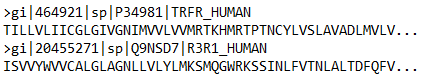
\includegraphics[width=\linewidth]{Figures/sequences.png}
	\caption{Sample FASTA input file containing two sequences from the \textit{7tm\_GPCRs} MSA.}
	\label{fig:sequence}
\end{figure}

\subsection{Embedding vectors and cosine similarity}
With FASTA input files containing two protein sequences, the embedding vectors and cosine similarity will both be extracted independently for analysis and visualization. By using the \textit{E}-score notebook as a starting point, modifications and new methods will be created to extract this information for a provided FASTA file and model.

Defined in the \textit{E}-score analysis\footnote{https://github.com/rgavigan/e-score} repository are methods to retrieve this data, such as \(get\_embedding()\).

\subsection{Data analysis}
Analysis of embedding vectors and cosine similarity to generate useful visualizations and perform statistical analysis on results will be done in the \textit{E}-score analysis notebook. The following tools will be used:
\begin{itemize}
    \item{Seaborn \autocite{Waskom:2021} and Matplotlib \autocite{Hunter:2007} for data visualization}
    \item{SciPy \autocite{Virtanen:2020} and NumPy \autocite{Harris:2020} for statistical significance testing}
    \item{Scikit-learn \autocite{Pedregosa:2011} for normalization}
\end{itemize}

% Heatmaps Figure
\begin{figure*} % Two column figure (notice the starred environment)
	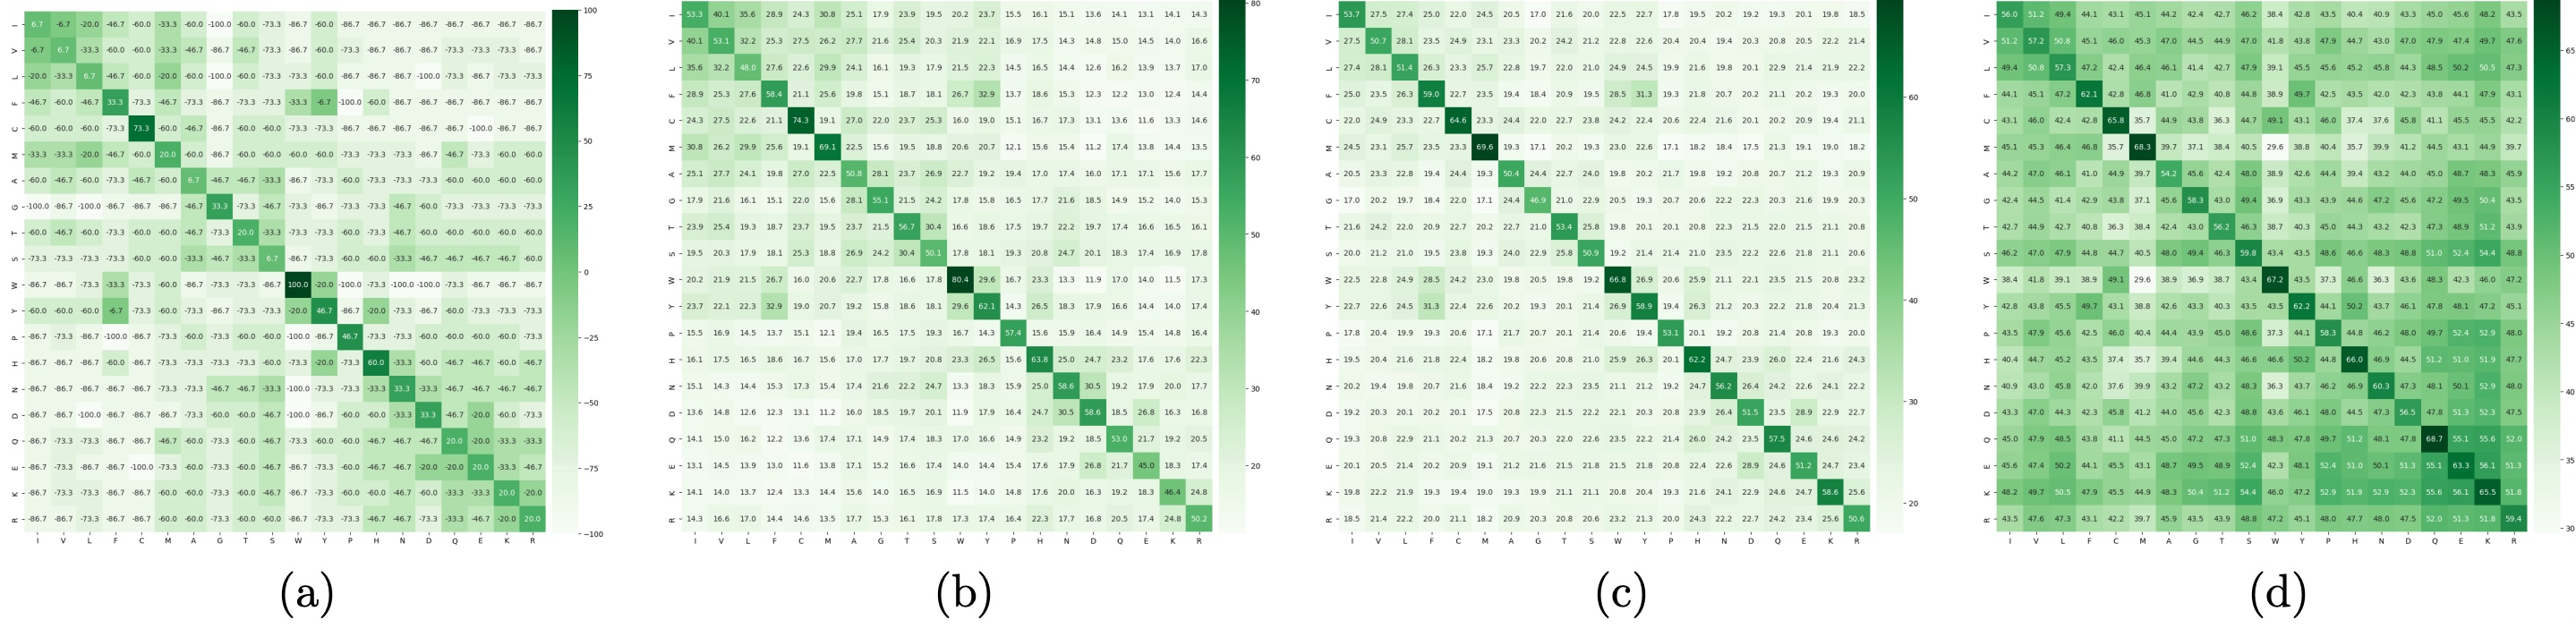
\includegraphics[width=\linewidth]{Figures/Escorematrices.jpeg}
	\caption{Heatmaps of (a) BLOSUM62 matrix (scaled to -1..1) and three aligned matrices of average E-scores for the NBD\_sugar-kinase\_HSP70\_actin MSA: (b) ProtT5-score, (c) ProtAlbert-score, and (d) ProtXLNet-score \autocite{Ashrafzadeh:2023}.}
	\label{fig:escoreheatmap}
\end{figure*}

\subsubsection{Embeddings}
Normalizing the embeddings generated between models to have a consistent scale and distribution is required prior to analysis. Common techniques for normalization to consider include min-max scaling, Z-Score standardization, and L2 normalization.

The distribution of normalized values can be visualized in multiple ways including histograms, kernel density plots, or box plots. Summary statistics (mean, median, deviation, range) may provide additional insight.

Correlations and differences between the embeddings can be visualized on a per-residue basis with heatmaps.

Statistical tests are required to validate and assess the significance of the visualized results. ANOVA, t-tests, or other means can be used to assess significance.

% Visualizing E-Score Dispersion
\subsubsection{\textit{E}-score}

To gain a deeper understanding of the \textit{E}-score results generated for the different embeddings as shown in Figure \ref{fig:escoreheatmap}, dispersion will also be visualized. By visualizing the standard deviation and range of the results for each embedding type, there will be more insight to draw conclusions from. This will help understand why cosine similarity mean results are mostly positive (0..1), and why different models generate broader or narrower average ranges.

% Modifying Parameters
\subsubsection{Modifying parameters}

By modifying different parameters and generating \textit{E}-scores for different combinations from insight gained by comparing different transformer models, further understanding of the primary factors contributing to performance will provide insight to improve embeddings. Examples of parameters that can be modified are alignment type, gap penalty, and gap extension penalty.

\subsection{Interpretation}
Through the visualizations and statistical analysis performed on embedding vectors and cosine similarity data, comparing properties that are present in stronger models (i.e. ProtT5) with weaker models will be a focus for interpreting the relevance of the analysis.

By benchmarking the models against one another and extracting features present in the stronger performing models, insight about why performance differences are present will be obtained and used to explain performance improvement approaches.

\subsection{Type of results}
Visualizations, statistical comparisons/tables, and inference using empirical findings to answer the research questions will be the anticipated results from this study.

\subsection{Challenges or threats}
Interpreting the meaning of embeddings is a challenging process because embeddings lack direct human interpretability due to their large dimensionality. Conducting appropriate statistical tests to validate findings and visualizing results to be human-readable is crucial.

Representative data for input sequences is necessary to minimize the chance of biased results.

%---------------------------------------------
%	NOVELTY AND IMPACT
%---------------------------------------------
\section{Novelty and Impact}

The anticipated result from this research is thorough insight into the \textit{E}-score method's results. These data-supported findings are expected to contribute significantly to the improvement of embeddings and the models that generate them.

There are three primary advancements that can be explored from the implications drawn from the results. These would serve as beneficial follow-up research to improve embedding performance, transformer models, and to apply the same advancements to Natural Language Processing.

% Improving Embedding Perforamnce
\subsection{Improving embedding performance}

From the novel insight gained about the properties that contribute to the performance of different protein embeddings, the performance of the embeddings can be improved for sequence alignment. This would be an application of the data-supported explanation for why different embeddings have different cosine similarity averages and ranges.

% Transformer Model Improvement
\subsection{Transformer model improvement}

The above insights can be used as a starting point to modify the architecture of the different transformer \autocite{Vaswani:2017} models such as the ProtTrans models ProtT5, ProtBert, ProtXLNet, and ProtAlbert \autocite{Elnaggar:2021}. This research can be extended to improve these models through different processes such as hyperparameter tuning and optimization.

The ProtT5 model, the best performing model from the ProtTrans project, would serve as a valuable model to fine-tune with the research implications drawn from this research. The ProtTrans GitHub repository\footnote{https://github.com/agemagician/ProtTrans/tree/master/Fine-Tuning} provides Jupyter Notebooks for fine-tuning this model for per-protein prediction, per-residue classification, and per-residue regression.

% Natural Language Processing
\subsection{Natural Language Processing}
The ProtTrans models available for the \textit{E}-score method are all derivations of Natural Language Processing models modified to work with the language of proteins, the 20 amino acids.

All of the above research (improving embedding performance and transformer models) can be repeated for Natural Language Processing contextual embeddings such as ELMo \autocite{Peters:2018}, BERT \autocite{Devlin:2018}, RoBERTa \autocite{Liu:2019}, XLNet \autocite{Yang:2022}, and T5 \autocite{Raffel:2020}. 

%---------------------------------------------
%	REFERENCES
%---------------------------------------------
\printbibliography % Output the bibliography

%---------------------------------------------
\end{document}